\chapter{Combat}\index{Combat}

\newcommand{\initiativechart}{

	\begin{tcolorbox}[title={Initiative Costs},arc=1mm,tabularx={lc}]

	\textbf{Action} & \textbf{Init. Cost} \\\hline

	-- \textbf{Striking} & \\\hline

	Heavy weapon & 8 \\

	Medium weapon & 6 \\

	Light weapon & 4 \\

	Drawing weapon & 2 \\\hline

	-- \textbf{Projectiles} & \\\hline

	Crossbow & 3 \\

	Improvised projectile & 7 \\

	Reloading & 2 \\

	Shortbow & 4 \\

	Thrown weapon & 4 \\\hline

	-- \textbf{Quick Actions} & \\\hline

	Defence & 4 \\

	Guard someone & 2 \\

	Keeping Edgy & 2 \\

	Moving & 2 \\

	Speaking & 2 \\\hline

	-- \textbf{Other} & \\\hline

	Use magic item & 8 \\

	Cast a spell & 3+level \\

\end{tcolorbox}

}

\begin{multicols}{2}

These life and death rolls are handled somewhat differently from other tasks. Let's start with an overview of the basic features then go over them again in more detail. 

You enter a dungeon, goblins are launching an attack from ahead.
You grab the dice and roll Initiative for the entire party.
The goblins have 9.
You (and therefore the party) have rolled 5.

Everyone adds their own bonuses to their Initiative score.
You get +2 for using a rapier, for a total of 7.
The party's dwarf has just +1 and acts on Initiative 6.
The goblins' spears give them a total of 12.

\paragraph{12:} The goblins spend 2 Initiative to run forward to attack.

\paragraph{10:} The goblins spend 4 Initiative to attack, and everyone defends against the onslaught of spears.
To simply defend, you spend 2 Initiative, putting you on 5.
\paragraph{6:} The goblins stab at the party again, going down to Initiative 1.
You decide to take your bruises and start swinging, without any proper defence.
\paragraph{5:} You hit back, killing your first opponent.
However, your heavy weapon costs 6 Initiative to take a swing, so you go down to Initiative -1.
\paragraph{2:} The rest of the party attack back.
Any goblin hit has to defend itself, putting it on Initiative -1.
\paragraph{1:} Any goblins who were not attacked begin another assault.
\paragraph{0:} The round ends.

A successful fight depends as much on proper pacing and timing as anything else.

Each \gls{round} you select your tactics anew and have a range of options for manoeuvres you can pull off.

\end{multicols}

\section{Basic Combat}

\begin{multicols}{2}

\subsection{Initiative}

At the start of each \gls{round} the leader of each group rolls $2D6$ and the result is the group's Initiative.\footnote{The ``party leader'', here means `whoever rolls the Initiative dice first'.}
Each character then adds their \textit{Initiative Factor} to get their Initiative Score.
The Initiative Factor is given by characters' Speed Attribute plus weapon modifiers.
If you roll 5 and have a Speed Bonus of 1, your Initiative Score is 6.

The \gls{gm} then counts downwards from the highest Initiative score.
When your number comes up, you can act.
Each time the character takes an action they pay a cost in Initiative -- once it reaches below 1 that character can no longer act.
Moving costs only 2 Initiative, while swinging an axe costs 6.
You can spend as much as you like, and even go down to an Initiative score of -5, but once the Initiative count reaches 0, the round ends.

Heavy weapons are generally more effective than Light weapons, but they cost 6 Initiative points to take a swing, while Light weapons cost only 4.

Heavy weapons are those with a Weight Rating of -1 or greater. Smaller weapons, those with a Weight Rating of -2 or less, and brawling attacks with fists, all count as light weapons.

\subsubsection{Quick Actions}

\Glspl{quickaction} can interrupt the usual Initiative priorities.
Any time someone attempts a Quick Action, they take their action immediately, even if they have a negative Initiative score.
If two characters interrupt the Initiative flow with Quick Actions then whoever currently has the highest Initiative Score goes first.

Quick Actions allow characters to guard someone as soon as they see an attack impending upon a friend, to defend against missile attacks, or to shout a few words.


\subsection{Attack}

To attack an opponent, you roll $2D6$ as usual, but only add your Combat Skill.
The \gls{tn} is 7 plus your opponent's Dexterity.

\subsection{Damage}\index{Damage}

If you hit, roll $1D6$ plus your Strength Bonus to determine Damage.
The Damage is then taken off the enemy's \gls{hp}.
Everyone has a number of \gls{hp} to withstand Damage. When your opponent is reduced to 0 \gls{hp}, they are defeated.

\subsubsection{Stacking Damage}\index{Combat!Stacking Damage}

Damage Bonuses cannot extend forever. If the Damage bonus ever exceeds +3 then 4 points of the bonus are replaced with a die. Therefore, what might usually be $1D6+4$ Damage becomes $2D6$ Damage.

This applies to all Damage, including magical Damage. It continues through all Damage Bonuses, so $1D6+9$ Damage would be simply $3D6+1$ Damage after conversion.

\subsection{Defence}

When the enemy attempts to hit you, roll for defence with your Dexterity at \gls{tn} 8 plus your opponent's Combat Skill.
Defending costs 2 Initiative and counts as a \gls{quickaction}, so it can be done immediately.

\initiativechart

\subsection{Movement}\index{Movement}

By spending two Initiative, characters can run as a Quick Action, acting before all other actions. Characters can run 3 squares plus their Speed Bonus during this time. This movement can be chopped up into any number of pieces -- once the Initiative is spent, a character with Speed +1 might run only one square, then 2 more, then 1 more square later.

Characters who spend the entire turn running can move 10 squares plus their Speed Bonus plus their Athletics Skill Bonus; so someone with Speed +1 and Athletics +1 would move 12 squares per turn of flat-out running.

\iftoggle{verbose}{
	\begin{tcolorbox}[title=Dicey Damage]

If you prefer your Dice in a more old-school format, you can easily give each weapon a different Damage die. Weapons which would normally inflict +1 Damage can instead roll their Damage as 1D8, while weapons with +2 Damage would instead leave players rolling 1D10, leaving weapons of +3 Damage to be replaced with a D12.

Whether the players are rolling $1D6+1$ for a dagger or 1D8, both have the same average of 4.5, so this system will not change things significantly. However, Stacking Damage occurs less often, and the die rolls will tend to swing more wildly to the highs and lows.

If you don't own a D14, then simply add +1 Damage to all Damage totals above +3.

+0 Damage should remain as $1D6$ and anyone with a Strength score of +4 should replace the bonus with a $D6$ as normal. Spells are unaffected.

	\end{tcolorbox}}{}

\subsection{Hit Points}

\index{Hit Points}Each character has a number of HP equal to 6 plus their Strength Bonus. Small gnomes typically have 4 HP while big, strong humans typically have 7. Losing even a single HP means the character has suffered serious Damage. A long fall might have broken the character's bone. A dagger could have slashed open several veins. Characters do not have many HP so losing even one is a serious matter.

\subsubsection{Healing}\index{Healing}
Characters heal a quarter their Hitpoints each week, rounded up.

\subsubsection{Death}
\index{Death}Once a \gls{pc} reaches 0 HP they must make a \index{Vitality Check}Vitality Check in order to stay alive. This is rolled at \gls{tn} 4 plus one for every negative HP level. For example, if someone with 3 HP left were to take a further 6 Damage, this would put their at -3 HP. That makes the \gls{tn} 7 for the Vitality Check.

A failed Vitality check means that the character is dead. A successful one means that the character is unconscious for the remainder of the scene but alive. At the end of the scene they can make further Vitality Checks to see if they wake up. When waking up, all actions relying on movement take a penalty equal to the number of HP beyond 0 the character has lost.

\glspl{npc} roll Vitality checks at a basic \gls{tn} of 7 instead of 4.\iftoggle{verbose}{\footnote{Traits such as Strength do not affect the Vitality check because in a way, they already have.  Stronger characters already have more Hitpoints, which has already kept them farther from death.}}{}


\end{multicols}

\section{Weapons}

\begin{multicols}{2}

Weapons are a great way of inflicting additional Damage, but they are an equally excellent way of defending oneself. Having a longsword to keep scary opponents at bay is always better than trying to nimbly dodge about. Longer weapons also grant a bonus to Initiative, representing the fighter's ability to hit opponents before they hit them due to the weapon's length.

Each weapons is rated for `Dam' (the Damage bonus), `Init' (the bonus to Initiative, generally through reach) and `Ev' (the weapon's Evasion bonus).

Each weapon has a Weight Rating, just like any item. For every point a weapon's Weight Rating exceeds its wielder's Strength Bonus, the wielder gains 1 Encumbrance, which subtracts from the character's Effective Speed as they move slower and swings the weapon slower. Weapons held in only one hand add +2 to their Weight Rating.

Finally, some weapons also have an in-built `Knack' -- a special ability they allow the wielder to use.
See page \pageref{knacks} for details.

\end{multicols}

\newcommand{\weaponschart}{
	\begin{tcolorbox}[arc=1mm,tabularx={p{.20\textwidth}p{0.07\textwidth}rrrp{.30\textwidth}}]
	\textbf{Light Weapons} & \textbf{Dam.} & \textbf{Init.} & \textbf{Ev.} & \textbf{Wt.R} & \textbf{Knacks} \\\hline

		Cudgel & +2 & \ 0 & \ 0 & -3 & Stunning Strike (page \pageref{stunningstrike}) \\

	Dagger & +1 & \ 0 & +1 & -4 &  \\

	Firepoker & +1 & +1 & \ 0 & -2 & Finishing Blow (page \pageref{finishingblow}) \\

	Knife & +1 & 0 & \ 0 & -4 & Precise Strike (page \pageref{precisestrike}) \\

	Log & +1 & -1 & \ 0 & -2 & \\

	Rapier & +1 & +2 & +1 & -2 & \\

	Rock & +1 & \ 0 & \ 0 & -5 & \\

	Javelin & +1 & +2 & \ 0 & -2 & \\\hline


	\end{tcolorbox}

	\begin{tcolorbox}[arc=1mm,tabularx={p{.20\textwidth}p{0.07\textwidth}p{.07\textwidth}p{.07\textwidth}p{.07\textwidth}p{.30\textwidth}}]

	\textbf{Medium Weapons} &  &  &  &  &  \\\hline

	Boulder & +3 & -1 & \ 0 & 4/6 & Finishing Blow Finishing Blow (page \pageref{finishingblow}) \\

	Chair & +1 & +1 & +1 & 1/ 3 & \\

	Club & +2 & +1 & +1 & 2/4 &  \\

	Great Axe & +3 & +1 & +1 & 3/5 & \\

	Great Sword & +2 & +1 & +2 & 3/5 & \\

	Large Rock & +2 & \ 0 & \ 0 & 4/6 & \\

	Longsword & +1 & +1 & +3 & 1/3 & \\

	Shortsword & +1 & +1 & +2 & -1/1 & Furious Blows (page \pageref{furiousblows}) \\

	Spear & +1 & +1 & +2 & 0/2 & First Strike (page \pageref{firststrike}) \\

	Quarterstaff & \ 0 & +1 & +2 & 0/2 & First Strike (page \pageref{firststrike}) \\

	Whip & \ 0 & +2 & \ 0 & -1/ 1 & \\

	Wood Axe & +2 & \ 0 & +1 & -1/1 & \\\hline

	\end{tcolorbox}

	\begin{tcolorbox}[arc=1mm,tabularx={p{.20\textwidth}p{0.07\textwidth}p{.07\textwidth}p{.07\textwidth}p{.07\textwidth}p{.30\textwidth}}]

	\textbf{Heavy Weapons} &  &  &  &  &  \\\hline

	Great Club & +4 & +1 & +1 & 5 & \\

	Giant Sword & +3 & +1 & +2 & 5 &  \\

	Poleax & +3 & +1 & +1 & 5 & First Strike (page \pageref{firststrike}) \\\hline

	\end{tcolorbox}

	\begin{tcolorbox}[arc=1mm,tabularx={p{.20\textwidth}p{0.07\textwidth}p{.07\textwidth}p{.07\textwidth}p{.07\textwidth}p{.30\textwidth}}]

	\textbf{Shields} &  &  &  &  &  \\\hline

	Bucklar Shield & +2 & \ 0 & +1 & -2 & Solid Defence (page \pageref{soliddefence})\\

	Kite Shield & +1 & \ 0 & +3 & 2/4 & Solid Defence, Dodge (page \pageref{soliddefence}) \\

	Round Shield & +1 & \ 0 & +2 & 0/2 & Solid Defence, Dodge (page \pageref{soliddefence}) \\
\end{tcolorbox}}

\weaponschart

\begin{multicols}{2}

\subsubsection{Light Weapons}\index{Light Weapons}

Light Weapons are those with a Weight Rating of -2 or less. People wield them in one hand only, without problem, and can slash or stab with them in flurries of blows, quickly. They require only 4 Initiative points to attack with, so while an axe is far more damaging than a dagger, a dagger can unleash a flurry of blows before a single axe swing has taken place.

\subsubsection{Medium Weapons}\index{Combat!Medium Weapons}

Swords, axes and all the regular weapons of warfare require a full 6 Initiative points to be swung. They grant excellent Combat Bonuses, often increasing the effects of all three Attributes. These weapons are the standard weapons which most people will be using throughout the campaign -- they cover the Weight Ratings from -1 to 4.

Medium weapons can be wielded in one hand, but with some difficulty, as this adds +2 to their Weight Rating. A great sword can certainly be held up by one hand alone, but it will move from a Weight Rating of 4 to 6, meaning that a normal human, with Strength +1, would suffer a -5 penalty to their Speed Bonus, and therefore Initiative. While this is a steep penalty to Initiative, the price can be worth the wielding of a shield with a weapon.

Anyone wielding a medium (or indeed heavy) weapon with a weight rating equal or greater than their racial maximum has an unwieldy weapon indeed, and suffers a -3 penalty to their Initiative.

\subsubsection{Heavy Weapons}\index{Combat!Heavy Weapons}

Giants, monsters and a few extremely strong humans have the ability to heft weapons so large that they can only be used with both hands together -- all have a Weight Rating of 4 or more.
They grant excellent Bonuses, but require 8 Initiative points to attack.

Anyone insane enough to attempt to use a large weapon one handed must suffer through a +4 increase in the weapon's Weight Rating, which would make such weapons prohibitively heavy for most people.

\subsection{Shields}\index{Shields}

Shields are a special type of weapon used almost exclusively to defend.
They have stats like any other weapon but with one important difference -- their Evasion bonus always adds to the Evasion Factor.\footnote{See below, page \pageref{stances}.}
This is true even if the character is using the Aggressive Stance.
Characters using a sword and a shield can add the shield's bonus to Evasion to their Evasion Factor while using the sword's Evasion Bonus and their Dexterity Bonus to Strike the enemy.

\end{multicols}

\newcommand{\armourchart}{

	\begin{tcolorbox}[arc=1mm,tabularx={lcc}]

	Armour & \gls{dr} & Weight \\\hline

	Elvish & 2 & -2 \\

	Padded & 2 & 1 \\

	Leather & 3 & 0 \\

	Chain & 4 & 1 \\

	Plate & 5 & 2 \\

	\end{tcolorbox}
}

\section{Armour}\index{Armour}

\begin{wraptable}{r}{.24\textwidth}

\armourchart

\end{wraptable}

\begin{multicols}{2}

Armour defends characters by lowering incoming Damage. In game terms, armours have a \gls{dr} rating which subtracts from Damage.

Armour can cover more or less of a character, and therefore comes with three ratings -- Partial, Complete and very rare Perfect armour. Partial armour covers the basics -- the character's chest and probably head, perhaps a basic arm-guard on top of that. Complete armour covers the full character -- almost. Complete armour, whether leather or plate, will come with a helmet, a neck-guard, gauntlets, shinguards, foot coverings and will overlap to protect the joints. Perfect armour is a rating used for certain creatures which have natural armour without weakspots (such as stone giants).

\subsection{Vitals Shots}\label{vitals}\index{Combat!Vitals Shots}

When attacking an opponent in armour, it is possible to make a shot so precise as to get a gap in a helmet, strike an opponent in the eye or slide a blade between overlapping plates. To get a Vitals Shot, one simply needs to roll high enough over the creature's regular \gls{tn} and all armour (meaning \gls{dr}) can be ignored.

For partial armour, anyone rolling a Margin of 3 (i.e. 3 points above the \gls{tn}) ignores the \gls{dr} from the armour. If the regular \gls{tn} is 8 then any roll of 11 or greater counts as a Vitals Shot. Complete armour requires a Margin of 5 to ignore the armour, so if the \gls{tn} were 10 then a Strike would require a total of 15 to bypass the armour. Perfect armour cannot be bypassed by a sufficiently high roll.

\iftoggle{verbose}{
\vfill\null
	\noindent\includegraphics[width=.9\linewidth]{images/Roch_Hercka/vitals_shot.jpg}
	\label{roch:vitals}
}{}

Many creatures have a \gls{dr} from natural armour, representing especially thick skin or some other immunity to Damage. Natural armour always counts as Complete armour unless otherwise specified, because it covers almost all of the body, but often leaves weak spots open such as the eyes or the kneecaps.

\iftoggle{verbose}{Vitals Shots not only provide incentive for people to push their Strike Factor as high as possible, even at the expense of their own defence.  It also provides an equalizer for weaker forces as even the most heavily armoured creature can be struck by a lucky blow.}{}

\subsection{Weight}

All armour has a Weight Rating, just like any other item. The Weight Ratings above are for Partial Armour. If anyone wears Complete armour the Weight is increased by 1, so Complete chain armour which comes past the knees, has a helmet and uses arm-guards, would have a Weight Rating of 2.

Armour also inflicts Fatigue very quickly, as mentioned above. Wearing armour in battle is a great idea, but characters attempting to sprint in full plate will find themselves unable to run before long.

\subsection{Perfect Strikes}

\index{Combat!Perfect Strikes}Rolling a \gls{natural} `12' in combat, i.e. rolling two 6's, means the roll was a Perfect Strike. A Perfect Strike is guaranteed to hit even if it doesn't reach the opponent's \gls{tn}, it ignores both Partial and Complete armour (covered below) and it grants +2 Damage.

\end{multicols}

\section{Advanced Combat}

\begin{multicols}{2}

With the advanced combat rules, \glspl{pc} have the option to change how they attack each round.
Those who are certain they can strike the shambling undead might focus more on defence than attack.
Others, hoping to bring down a massive basilisk in one hit might put all their resources into an accurate attack with a high Initiative score.

To keep track of all this, we track three `Factors'.  The \textit{Strike Factor} is to attack, the \textit{Evasion Factor} to avoid being attacked, and the \textit{Initiative Factor} to add to Initiative.

\subsection{Stances}\label{stances}
\index{Stance}

The Dexterity Bonus can be assigned to either the Strike Factor or the Evasion Factor.
This includes the weapon bonus.
Someone with a Dexterity Bonus of +1 and a longsword would have a total Dexterity Bonus of +4, and can assign that to either Strike or Evasion.

This bonus cannot be picked apart - the entire thing must go towards only one of these two Factors.

\subsection{The Combat Bonus}

The Combat Skill can be added piece by piece to any of the Combat Factors.
Those with Combat +1 can put it on Strike, Evasion or Initiative.
Those with Combat +2 allows you to place +1 on Strike and +1 on Evasion, or +2 on Initiative, or any other combination.

The character sheet has a space for coins on top of the Combat Factors so you can place your Dexterity Bonus and the Combat Skill on top to remember what you have.

At the end of the round, the Combat Factors reset, and everyone chooses what they want to do again.

\iftoggle{verbose}{

In all cases there is an optimal configuration which will itself depend upon the enemy's placement of resources.\footnote{Players and \glsentrylongpl{gm} are free to cover their coins with their hand until everyone has placed their resources for the round.}

}{}

\subsubsection{Aggression}

Animals use a Skill called `\index{Aggression}Aggression' to Strike -- Aggression works exactly like the Combat Skill but only adds to the Strike Factor, and never to Initiative or Evasion.

\iftoggle{verbose}{
	\noindent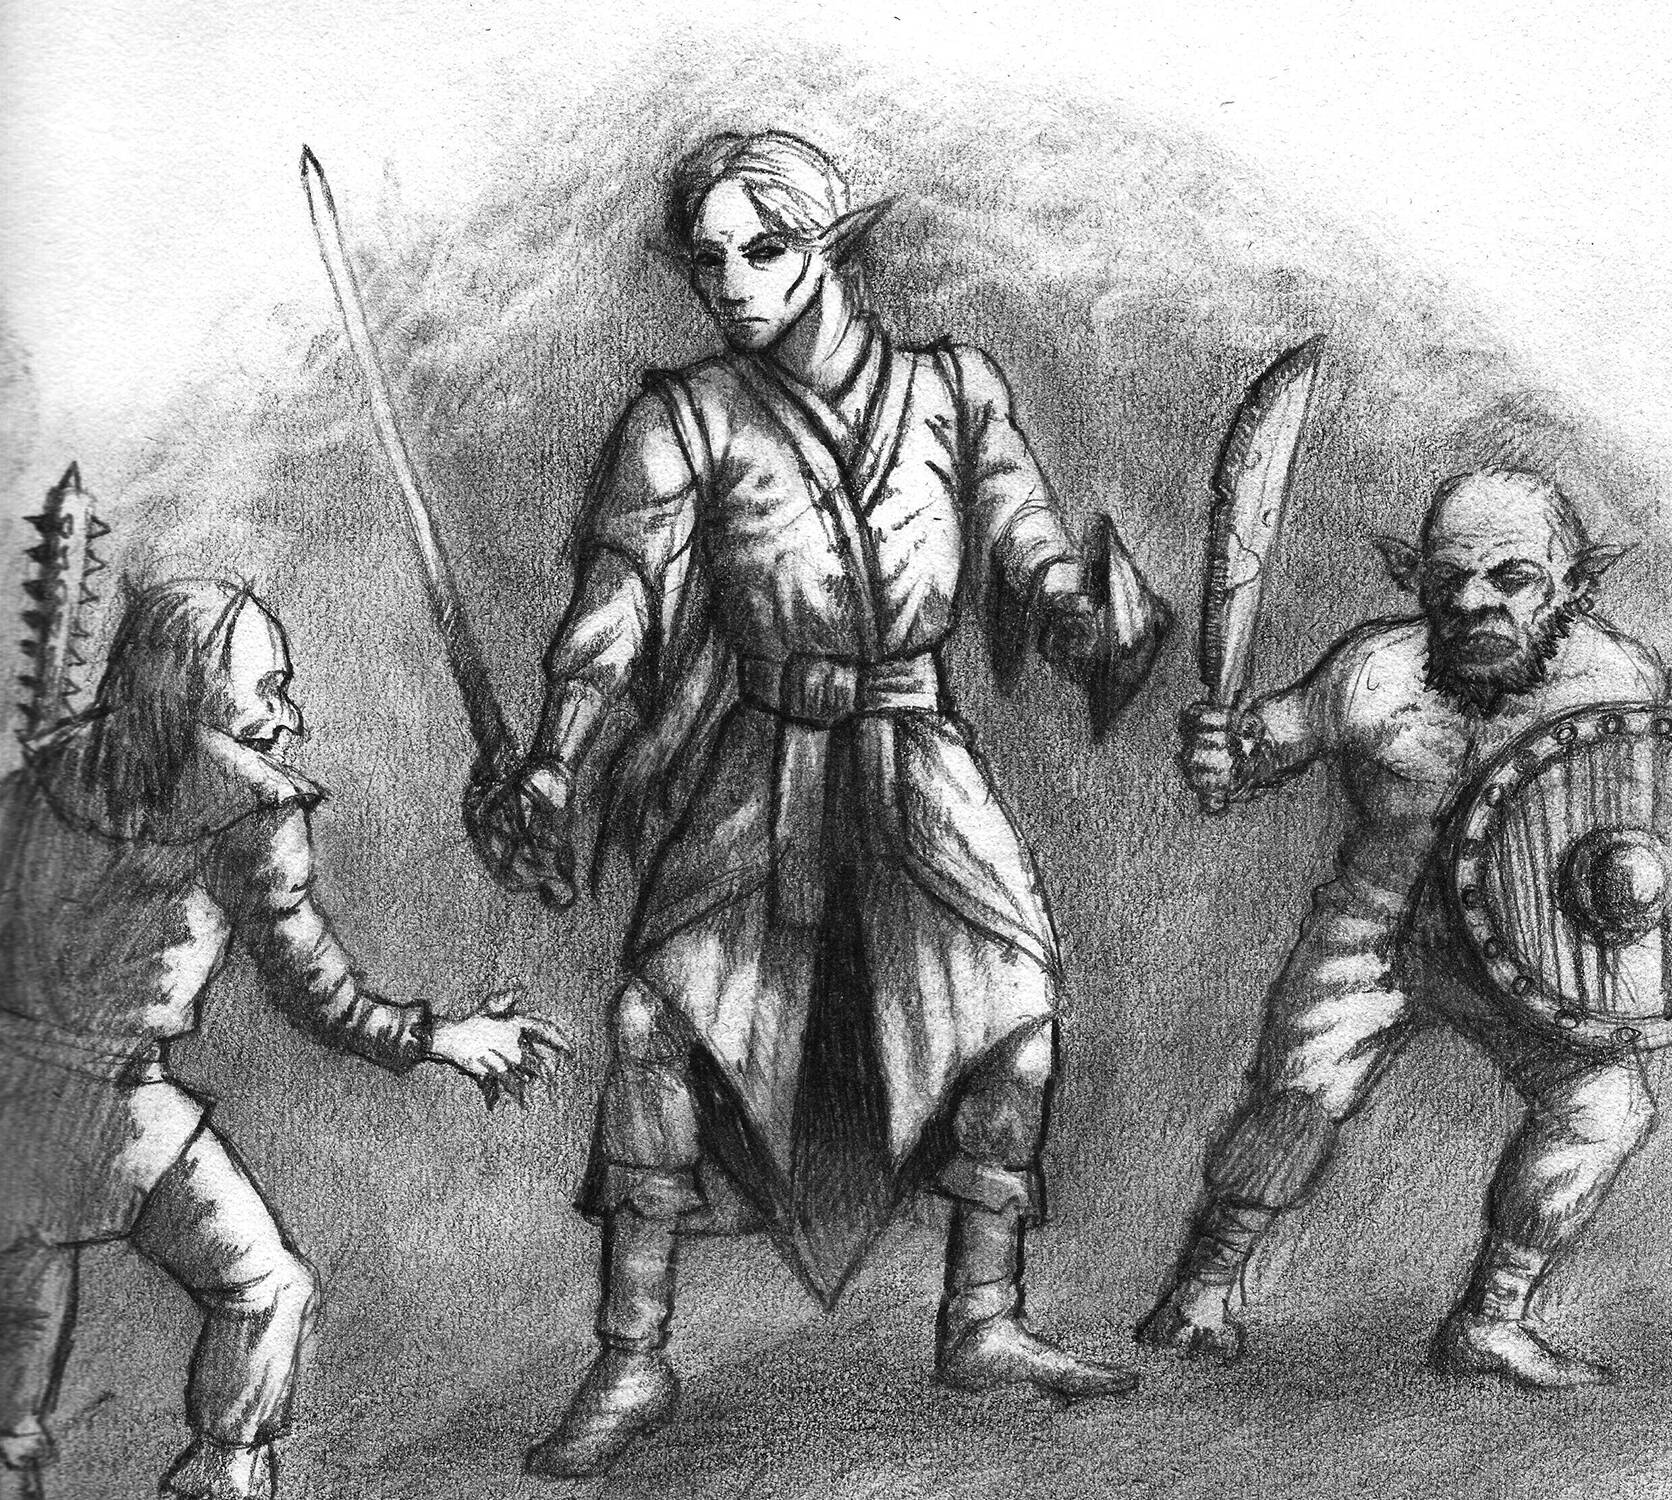
\includegraphics[width=.8\linewidth]{images/Roch_Hercka/stances.jpg}
	\label{roch:stances}
}{}

Characters can attack in an \textit{Aggressive} or \textit{Defensive} stance. This system takes the Defensive stance as default -- the Dexterity Bonus is added to the Evasion score to keep the character safe. However, a character can forego safety for additional combat ability and add the Dexterity Bonus to Strike should they wish. Any Bonuses to Evasion from weapons also add to the Strike Factor. The score cannot be divided between the two -- the Stances are an `all or nothing' affair. Delicate decisions concerning priorities require the Combat Skill, which can be added one piece at a time to any of the Combat Factors.

If a character's Evasion score ever becomes negative, it applies to the Strike score when using the Defensive Stance. It is possible to swap it back by taking the Aggressive stance but this almost guarantees that opponents will hit the character every time they strike.

\end{multicols}

\section{Fate Points}\label{fate_points}\index{Fate Points}

\begin{multicols}{2}

\begin{wraptable}{O}{.17\textheight}

	\begin{xpbox}{C}
		Base FP & Regeneration \\\hline

		5 & 2 per scene \\

		10 & 4 per scene \\

		15 & 6 per scene \\

		20 & 8 per scene \\
	\end{xpbox}

\end{wraptable}


At this point you might be wondering how anyone is going to survive past their first battle. 6 or 7 HP is not a lot when the Damage is often $2D6$ or higher. The mechanism which saves the plot-important character is \gls{fp}. Every time someone would lose HP, the character marks off \gls{fp} instead and it is stipulated that the attack in fact misses, because the gods have fated this person to live another day.

Everyone in the world begins with 5 base \gls{fp}. This is then modified by their Charisma Bonus, so someone with Charisma -2 starts with 3 \gls{fp}. The difference between the \glspl{pc} and the \glspl{npc} is that \glspl{pc} start play with a full alotment of \gls{fp} at the beginning of each adventure. \glspl{npc} start with none, but regain \gls{fp} at the end of each scene as usual. As a result, most \glspl{npc} effectively have 0 \gls{fp}. The \gls{gm} can mostly ignore \gls{npc} \gls{fp} and Damage will be applied directly to \gls{npc} HP.

\subsection{Regaining Fate Points}

At the end of each Scene, players regenerate 2/5ths of their Fatepoints.  Those with 5 Fatepoints total regenerate 2 temporary Fatepoints, and those with 10 Fatepoints regenerate 4 temporary Fatepoints, and so on.

While \glspl{npc} begin with 0 \gls{fp}, they too regenerate the normal amount each scene. In this way, an \gls{npc} might accumulate quite a number of \gls{fp}, and when some climactic end scene arises where the \glspl{pc} finally confront them, they will have a harder time of it, because the \gls{npc} has now become plot-important enough to merit some plot immunity, just like them.

One exception here is creatures without a Charisma Attribute. Animals, undead and other creatures without any Charisma Bonus can never store \gls{fp} except through the use of Magic.

\end{multicols}

\section{Fatigue}

\begin{multicols}{2}

\label{fatigue}\index{Fatigue}Fighting, running and swimming can really take it out of you, especially when wearing heavy armour. Characters gain Fatigue points for exerting themselves, and if they accrue too many then they will quickly start to become ineffective.

Below the character's HP bar are spaces for Fatigue Points to be gained. Once the character has more Fatigue Points than their current HP, they take a -1 penalty for every Fatigue Point in excess of their HP.  This might happen because the character has, say, 6 HP but gains a total of 8 Fatigue Points, and then gains a -2 penalty to all actions. But it might also occur because the character has 4 Fatigue Points and then Damage reduces their to only 2 HP, leaving them with a -2 penalty to all actions yet again.

Characters may reach a maximum penalty of -5 due to Fatigue Points, after which they die. If the character is accruing Fatigue Points from running or wrestling, they would normally simply pass out at this point, but if they are gaining Fatigue from swimming or bleeding, the character will almost certainly just die.

Fatigue Points cannot be mitigated with \gls{fp}. Characters who can luck their way out of being shot by arrows and roasted by dragons can quite easily be punched and dragged away, or collapse after a long run.

\subsection{Gaining Fatigue}

\paragraph{Bleeding} If the character has lost HP to piercing or slashing weapons they should gain Fatigue Points equal to the number of HP lost. These Fatigue Points are marked with a `B' instead of the usual dash across a box and are healed at a rate of one per day rather than the usual, faster rate. If the bleeding is not stopped, the character should bleed for the same number of points \ minus one on the next scene until they are dead or the bleeding has stopped on its own. The \gls{tn} to stop the bleeding is always 6 plus the number of Fatigue Points being lost on the current scene.

\paragraph{Climbing} Every 2 squares climbed upward inflicts 1 Fatigue Point.

\paragraph{Encumbrance} Each point of Encumbrance inflicts 1 Fatigue Point at the end of the scene.

\paragraph{Fighting} Each \gls{round} of Combat inflicts 1 Fatigue Point.

\paragraph{Holding Breath} Each \gls{round} a character holds their breath inflicts 1 Fatigue Point. This Fatigue is applied each \gls{round} rather than at the end of the scene.

\paragraph{Marching} Every mile of marching inflicts a Fatigue point.

\paragraph{Starving} Each meal skipped inflicts 1 Fatigue point plus the character's Strength Bonus (minimum of 1) for the first day and 1 Fatigue Point per day thereafter. Each day without water inflicts 3 Fatigue Points. These Fatigue Points are marked with an `S' and do not heal until the character gains some appropriate sustenance.

\paragraph{Swimming} Each \gls{round} spent swimming inflicts 1 Fatigue Point. This is in addition to holding one's breath, if the character is swimming underwater and unable to breathe while there.

\paragraph{Wearing armour} All armour adds a number of Fatigue points equal to the armour's Weight Rating. As usual, the Weight Rating is 1 higher for Complete Armour.

Fatigue Points are healed extremely quickly. In fact, during most \glspl{round} they will be healed faster than they are accumulated. Since they are both gained and healed at the end of the scene, \gls{gm} should look at the number of Fatigue Points that will be gained and healed and if there are none on balance then Fatigue can be ignored for yet another scene. Fatigue comes into play during connected scenes of continued endurance and action, or when PCs are attempting to see how long they can swim against an underwater current while wearing full plate armour. Or possibly, and quite rarely, Fatigue comes into play when a tiny, weak character attempts to do everything while wearing full plate armour.

\subsection{Healing Fatigue}\index{Resting}

\paragraph{Short Rest} Any scene which ends with characters resting allows them to heal 3 Fatigue Points plus their Strength Bonus, so a character with a Strength Bonus of +2 would heal 5 Fatigue Points.

\paragraph{Long Rest} Any full night of rest allows characters to heal 5 Fatigue Points plus their Strength Bonus.

\iftoggle{verbose}{
	\begin{exampletext}

	The next morning the trio gave a wide berth to the area between the fallen village and the mountain, in the hopes of avoiding attack from the rear.
Unfortunately there was little they could do to hide themselves, and a band of hobgoblins from the village were following them.
The trio had reached halfway up the mountain by this point but the hobgoblins were faster than them, and stronger.
Thenton thought for a moment about abandoning Hugi if there was a problem - his little dwarvish legs were no good for sprinting. Of course Hugi's death would not buy them much time, and Arneson would never stand for it. No, they would have to stick together to survive.

	The trio climbed for a while longer, looking back every few moments to note how close the hobgoblins were behind them. An ogre was among their ranks, so they must have come from a very deep cavern.

	Looking back, the enemy was nearing and everyone was out of breath. Arneson suggested a rest to make sure they would be ready for the fight - they could fight downhill against an enemy fatigued from walking upwards. He calmly got out the rations - some cheese, smoked pork, oatcakes and a flaggon of wine.

	\noindent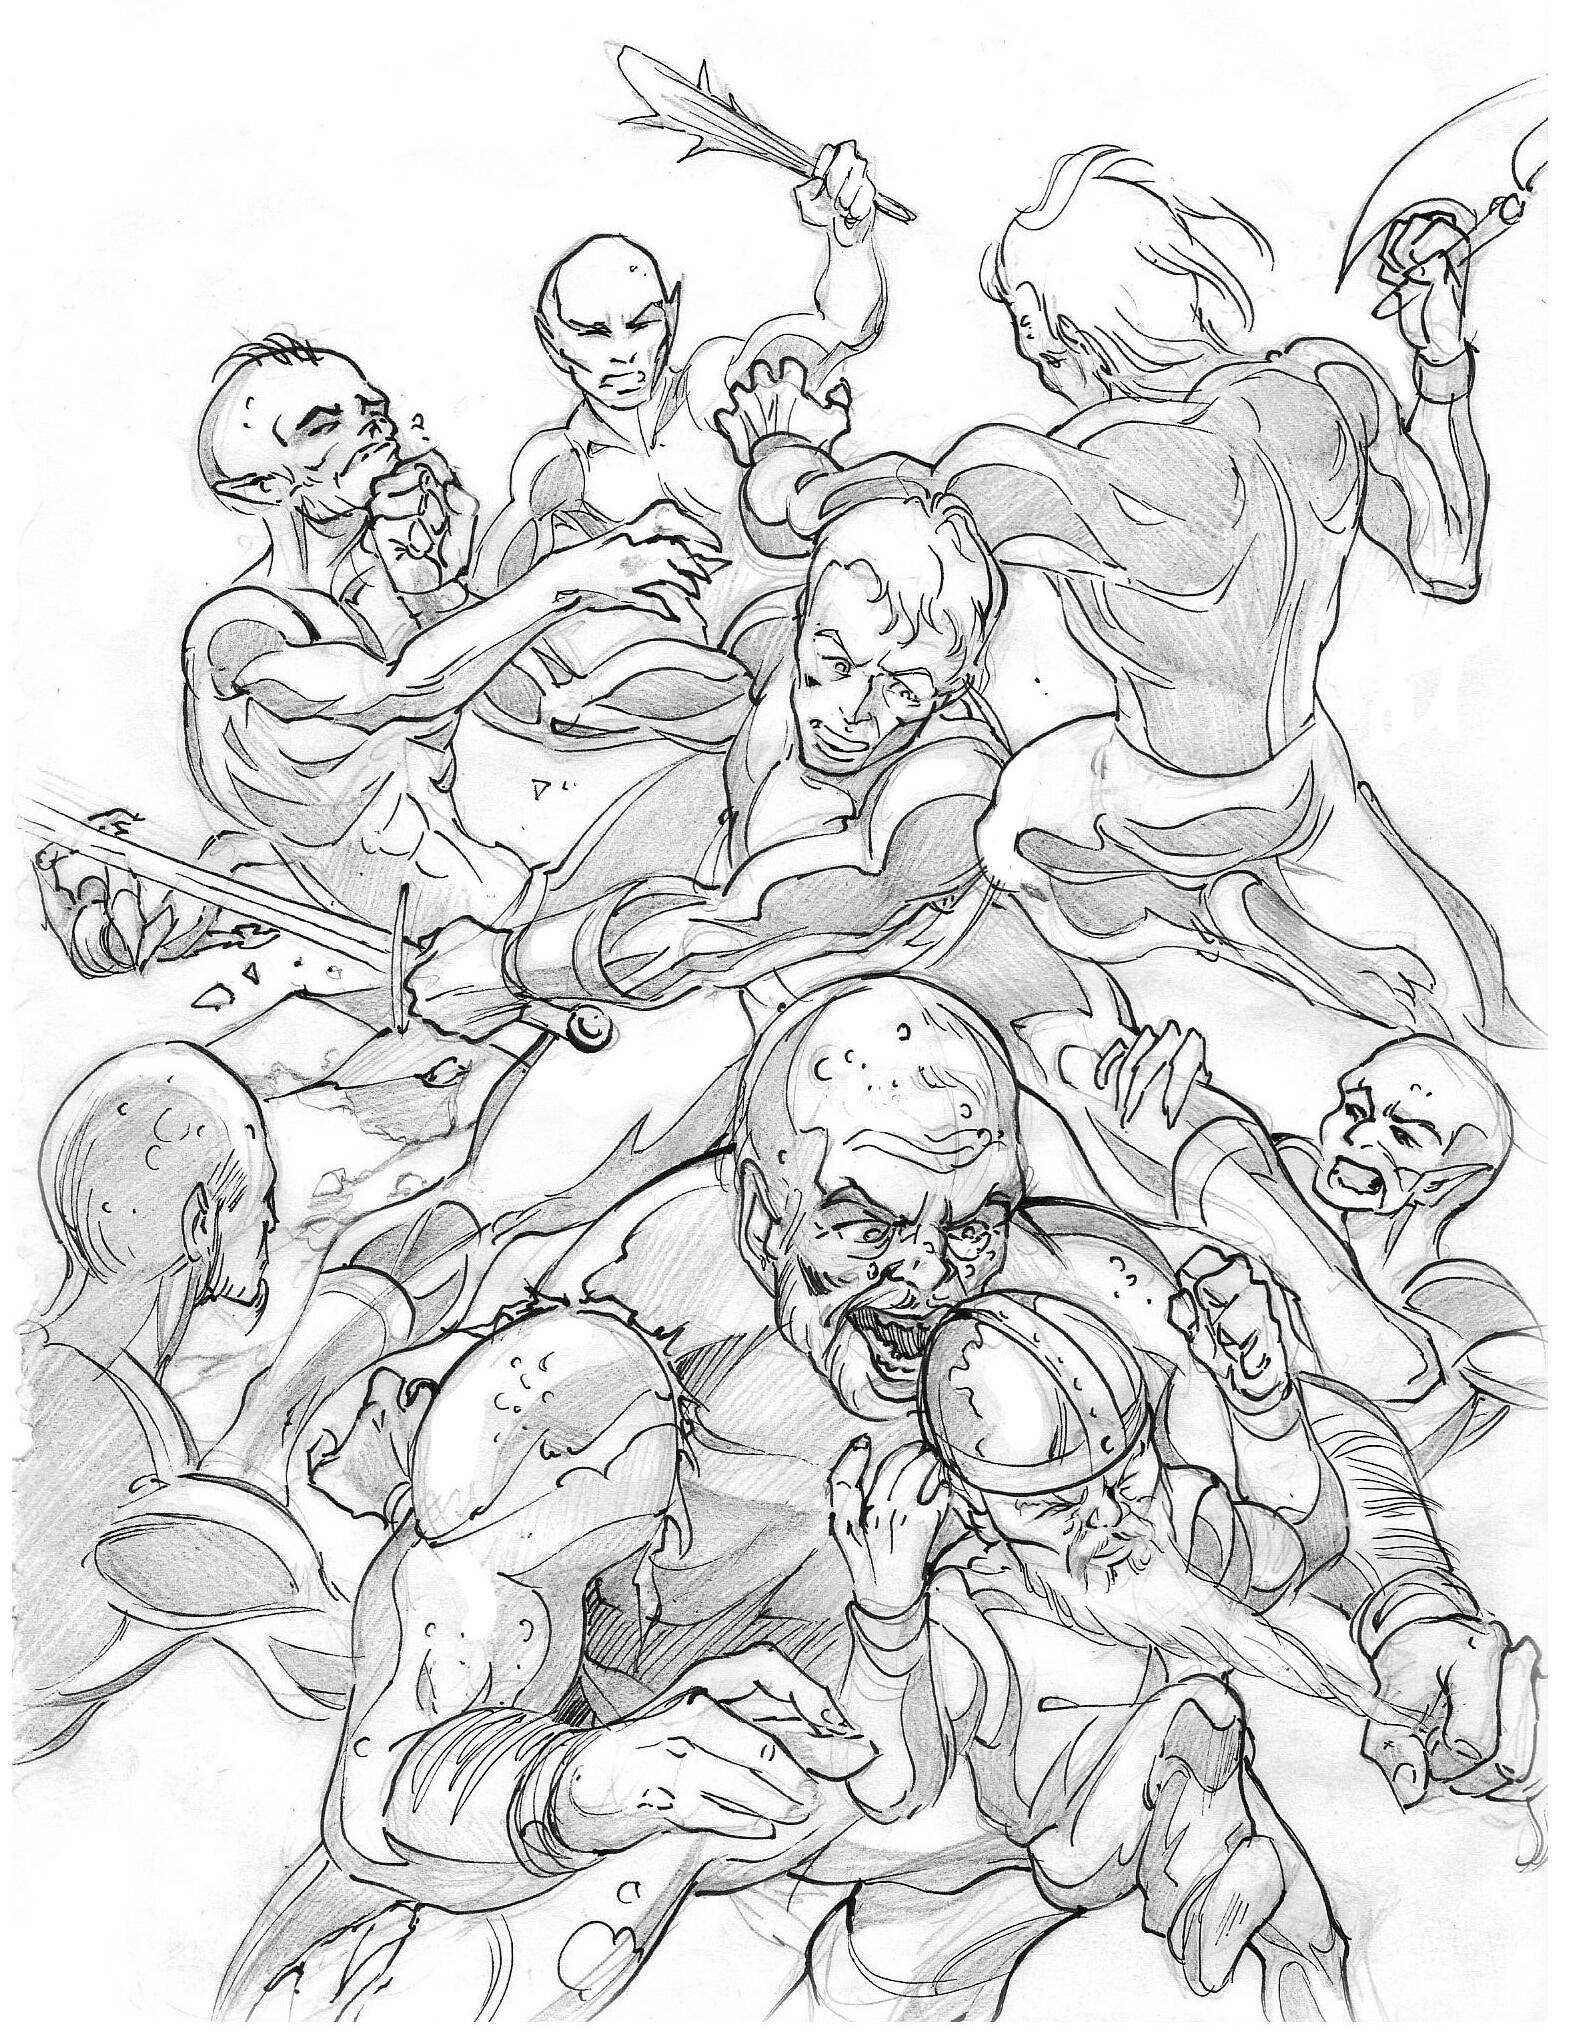
\includegraphics[width=\linewidth]{images/Boris_Pecikozic/nura_brawl.jpg}
	\label{boris:brawl}

	``May as well have the best of the rations now, eh, friends?'', Arneson said while smiling, and they slowly masticated their age-hardened meal and tried to smile back as the nine foot monstrocity which was so recently a man made its way up to them, pounding its great feet up the mountainous slopes, surrounded by half a dozen hobgoblins, each the size of a broad-shouldered man.

	As the hobgoblins neared the plateau where the trio sat they began to make their war cries, but Arneson just sat and ate his last oatcake slowly. They began to sprint upwards across the rocky ground.

	The \gls{gm} decides that since the players have the higher ground, they will receive +1 to all rolls until the hobgoblins can reach slightly higher ground - probably after the first action.
One of the players must roll Initiative, so Arneson's player take the dice and rolls, producing a `5'.
Each character's Initiative Bonus adds to this separately, so Thenton's Initiative of +1 gives him a total of 6; Hugi's Initiative of +0 gives him a total of 5 and Arneson's Initiative Bonus of +2 makes his total 7.
The group then gain +1 each due to the higher ground.
Meanwhile, the hoboblins have rolled a `5' for their Initiative as well.
The hoboblins each have a +1 bonus to Initiative and the ogre has a +0 bonus.

	The \gls{gm} knows the highest Initiative total is somewhere under 9 so she calls out,

	``Ten! The hobgoblins gather at the base. Nine! They cover their faces with their weapons and gang together. Eight! They push forwards and ....''

	``Eight!'' shouts Arneson's player. ``I'm going at eight! \ I'm going for the ogre - you said he was unarmoured so we should be able to take him down with a couple of good hits''.


	Arneson's player needs to roll an 8 to hit the ogre, so he rolls and adds +1 for his Combat Skill. His total is `11' and he hits. He has already rolled his damage die at the same time. It landed on a `2'. He adds +2 for his Strength and +1 for the sword's Damage bonus for a total of 5. The ogre shrieks in pain as Arneson's sword sticks in. Arneson's action took 6 Initiative points so he goes down to `2', and the hobgoblin has spent 2 Initiative to defend himself.

	``Seven!'', she cries. Thenton's player jumps in. He only deals $1D6+2$ Damage but he has a much better Combat Skill of +2. He rolls to Strike but misses the ogre with a `5'. His Initiative score reduces to 1, and he reduces the hobgoblin's from 6 to 4.

	``Six!'', beckons the \gls{gm}, and starts to describe leering hobgoblins stabbing at everyone's feet from the base of the great stone step the trio are sitting on. She gives them each a -1 to attack due to occupying the lower ground.

	A hobgoblin hits Arneson, so he spends 2 Initiative to attempt to Dodge. Arneson rolls a 7 but the \gls{tn} is 10.
The hobgoblin's Strength is +2 and the battle axe adds +3 Damage for a total of +5.
4 of the Damage is replaced with a die, so the hobgoblin is rolling $2D6+1$ Damage.
The total is 6.
Arneson's player first reduces that by his chainmail's \gls{dr} of 4, leaving 2 Damage.
Instead of taking that Damage he marks off 2 \glsentrylongpl{fp} and declares that the attack in fact misses.

		Hugi finally releases his crossbow, but in all the confusion misfires. He's down to Initiative 1.

		\needspace{3cm}
		\begin{wrapfigure}{r}{.3\textwidth}

			\begin{tabularx}{.3\textwidth}{c|X}
				\setcounter{enc}{12}

				8 & Arneson deals 5 Damage to a hobgoblin. \\

				7 & Thenton misses. \\

				6 & Most hobgoblins attack. \\

				5 & Ogre grabs Hugi, then runs away. \\
				4 & Two hobgoblins attack. \\


			\end{tabularx}

		\end{wrapfigure}

	``Four!'', shouts the \gls{gm}, then she smiles. The next hobgoblin attacks and Arneson rolls a 5 -- that's a failure with a Margin of 4, so it bypasses his chainmail. The axe is coming down towards his unarmoured shin-bone and the Damage rolled is 9. He marks off his last 9 \gls{fp} rather than taking any Damage. Any further Damage is coming straight off his \gls{hp}.

		``The ogre pushes forward with its club then reaches out to grab Hugi. Roll at \glsentrylong{tn} 9''.

		Hugi's player isn't happy, as that is enough to hit him, or in this case grab him. In fact with his crossbow out rather than a defensive weapon, he'll have a hard time defending himself.

		The ogre reached forward, grabbing Hugi by the beard and pulling him back through the horde of hobgoblins and out from the protection of his companions.

		The other players want to attack the ogre, but he's making a movement action - these count as Quick Actions so they are allowed to operate before other actions. Hugi disappears behind the crowd. The ogre's Initiative reduces to 0 and he is done for the \gls{round}, but Arneson and Thenton each have one action left.
	\end{exampletext}

}{}

\end{multicols}

\section{Complications \& Manoeuvres}

\begin{multicols}{2}

\subsection{Complications}

\subsubsection{Blindness}

\index{Blindness}\index{Combat!Blindness}Fighting while blind is no fun -- your opponent can see you coming, and you can't see them. Blinded opponents suffer a penalty equal to -8 plus their Wits and Vigilance Bonuses with a maximum penalty of -6. For example, a character with With -1 would receive a -9 penalty to attack, except that the maximum penalty is -6. Someone with Wits +1 and Vigilance +3 \ would suffer a -4 penalty to attack because both reduce the basic penalty of -8.

This penalty only counts when one side of a fight is blind. When both sides are blind, we use the Darkness Fighting rules below.

While fighting blind, if the dice make a \gls{natural} roll equal to the number of people on their side (including themself) then they hit a companion. If the character is fighting with just one companion then there are two of them and they hit a companion on the roll of a 2. If they are part of a group of 5 people, any roll of 5 or under means they have accidentally hit a companion. Companions who are are accidentally hit can attempt an Evasion roll by rolling with their current Evasion Factor against \gls{tn} 10; failure implies normal Damage from that attack. It is quite possible to kill a companion while fighting blind.

\subsubsection{Darkness}\label{darkness}\index{Darkness}

Fighting in the darkness, or just twilight, can give a distinct advantage to those with sharper senses.
Those who retain some basic vision while their opponents have none are in a similar situation to fighting a blinded opponent.
However, when both sides suffer from the darkness, the battle changes very little.
Neither side can hit very accurately, but then neither side can dodge or parry very well either.

When fighting in the dark, each side receives a penalty to attacking the other equal to the difference between their respective Wits + Vigilance totals, up to a maximum of -6.

For example, a human guard has caught a room full of elves with stolen goods. Thinking quickly, one of the elves douses the room's only lantern. The human has a Wits Bonus of -1 and no Vigilance Skill. The elves have a minimum Wits of +1 and many also have the Vigilance Skill; that means the elves will receive a +2 bonus to striking the guard and those with the Vigilance Skill will receive a higher bonus.

Deep darkness can provide a maximum penalty of -6, while twilight is limited to a penalty of -3.

\subsubsection{Passing Attacks}\index{Combat!Passing Attacks}

When someone is attempting to run past others, they have some opportunity to hit when the character is passing. This can be any normal attack, but counts as a Quick Action, jumping ahead in the Initiative Score. The attack costs the normal amount of Initiative.

\subsubsection{Spell Casting in Combat}\index{Combat!Spell Casting}

Spell casters are assumed to be focussing on their spells and using both hands for that purpose rather than weapons. They use their Wits for the Initiative bonus rather than Speed and receive no Combat Skill Bonus to Evasion -- they only use their basic Dexterity score.

Casting one-handed is possible, but difficult. Any roll the spell requires receives a -2 penalty. If the spell requires no roll then it is assumed it requires no hand movements and therefore gains no penalty. Casting one-handed allows the caster to hold a weapon in the other hand, for either defensive or offensive purposes.

Spell casters who wish to both attack and cast spells within the same \gls{round} must use the lower of their Speed and Wits score when determining Initiative. They can then use their full Combat Skill Bonus for the \gls{round} to add to the Combat Factors but cannot take their Initiative Factor higher than their Wits Bonus.

Switching away from one's focus on spells or martial combat must be decided at the start of the \gls{round} -- mages who are not mentally prepared to cast spells or use a sword cannot do so at a second's notice.

\subsubsection{Trapped or Entangled}

Characters caught in mud, who slip over, or get shackled to a spot cannot move or dodge nearly as well as they could.
They cannot take any Quick Actions except speaking, and receive no benefits from their Dexterity Bonus or the Knack: Fox Hop.

\subsubsection{Falling Prone}\index{Prone}\label{prone}

Characters who fall over lose their ability to defend themselves, as above.  However, they can get up at the cost of 2 Initiative by using up their movement action.  If they've already moved this \gls{round}, they have to wait until the next \gls{round}.

\subsection{Manoeuvres}

\subsubsection{Brawling}\index{Combat!Brawling}\index{Brawling}

Punches and kicks all use the Combat bonus. Such attacks inflict Fatigue Damage. Everyone gains a \gls{dr} against Brawling Damage equal to their Strength Bonus, which stacks with armour (\gls{dr} cannot be negative). This counts as Complete armour, so hitting someone in Partial chainmail with a \gls{tn} of 8 and a Strength of +1 would mean they have a total \gls{dr} of 6. However, an attack score of 11 would mean that the Partial armour's \gls{dr} could be ignored, leaving only a \gls{dr} of 1. An attack score of 13 would ignore both types of \gls{dr}, leaving nothing at all. Attacks which bypass a body's natural armour count as normal Damage as such attacks might hit vulnerable locations such as the eyes or crotch or twist an opponent's arm till breaking point.

\subsubsection{Blind Rage}\label{blind}

\index{Blind Rage}Weapons can grant a bonus to the wielder's Evasion Factor because the wielder is keeping people at bay with it -- a spear might be waved in an opponent's face in a threatening manner or a sword might be on the ready to attack if someone gets within its range. However, this marvellous defence only works against people who care about being hit. Anyone can choose to attack someone while ignoring their opponent's weapon's bonus to Evasion; the penalty is simply that the opponent can choose to make a single Sneak Attack immediately. This counts as a Sneak Attack, gaining +4 to hit and +2 Damage.\footnote{See page \pageref{sneakattack}.}

\subsubsection{Drawing Weapons}

\index{Combat!Drawing Weapons}Drawing a weapon costs 2 Initiative if it is placed in an easy place to draw, like a scabbard on the side of a belt. If a character holds weapons on the back or in a bag, it costs 8 Initiative to remove them. If a knife's stuffed inside a pack, the \gls{gm} may stipulate a number of \glspl{round} required to draw the weapon.

\subsubsection{Flanking}\label{flank}

Attacks from someone's anterior side gain a +2 Bonus.  Anyone caught alone is in more danger than they would be, due to opponents attacking from all side.

\subsubsection{Grabbing \& Grappling}\index{Combat!Grappling}

\paragraph{Grabs:}

A grapple always starts with a grab.  A grab is a normal roll, made without any benefits from weapons.  If successful, the character has grabbed an opponent.

Once two people are grappling, neither can move and so both can be struck as per a Sneak Attack by anyone nearby.

\paragraph{Grapples:}

Once two people are caught in the grapple, either can make a grappling roll at the cost of 4 Initiative.  They can then roll with double their Strength, plus their Strike factor, against 7 plus the enemy's Evasion score.

A successful roll implies the character can break the grapple and move freely, or can inflict $1D6$ plus their Strength Bonus in Damage.

\subsubsection{Guarding}\index{Guarding}

If you guard someone by standing in front of them then all attacks have to go through you first.\footnote{This includes missile attacks only if you could otherwise evade them.}  Any enemy making a successful attack on you can choose to damage you, or to make another roll (as a free action, costing no Initiative) at their real target.

Guarding costs 4 Initiative, as the character must both focus on helping a companion and focus on their own defence.
To put it another way, guarding someone costs 2 Initiative, and defence costs 2 Initiative as normal.

\subsubsection{Half Swording}\index{Combat!Half Swording}

It is possible to hold a sword by the blade and use the guard to bludgeon one's opponent. This manoeuvre allows the weapon's Speed Bonus to be added to its Damage instead. It takes 2 Initiative points to change how one holds the sword.

\subsubsection{Holding Off}\index{Combat!Holding Off}

Anyone can wait to see what the battle brings -- the character simply lowers their Initiative and can jump in at any point, acting at one Initiative higher than a declared action.

For example, someone might hold off their action at Initiative 5. They wait for the enemy to attack at Initiative 3 and notices that one of them is attempting to use a magical item. Immediately they retroactively performs an action at Initiative 4.

\subsubsection{Keeping Edgy}\label{edgy}\index{Keeping Edgy}

The character can take a moment to note their \index{Dodge!Long-range}long-range surroundings, including archers and potential spell casters.
This takes only 2 Initiative points and for the rest of the \gls{round}, any time the character is being fired upon in combat they can use their basic Speed Bonus in a resisted action to leap out of the way of an incoming missile or targeted spell, such as a fireball.
Spells which simply target people by gaze or magical effects such as Polymorphing are unaffected.

\subsubsection{Ram}\index{Combat!Ram}

In combat, it is possible to scare, push and stab at someone to force them to move backwards. The attacker spends 3 Initiative points. The defender can either attempt to resist, or can simply acquiesce and move back. When moving back, targets are pushed back 2 square; the attacker's Strength adds to this and the opponent's Strength decreases it. Characters can sacrifice the use of 1 point of Strength to push back an additional person.

Those who resist must also sacrifice 3 Initiative. A resisted Strength + Combat Skill check is made. Successful resistance means that the defender is not pushed back.

A \textit{Ram} action must employ normal movement, and cannot move any character farther than their normal movement.  Characters who have been rammed but are unable to move far enough back fall \textit{prone}.\footnote{See page \pageref{prone} for details on falling prone.}

\subsubsection{Sneak Attacks}\label{sneakattack}\index{Combat!Sneak Attack}

When taking someone by surprise, the attacker gains a +4 bonus to the attack and a +2 bonus to Damage. Opponents cannot use any Evasion bonuses from Dexterity, weapon Bonuses or the Combat Skill.

Sneak Attacks also gain a penalty equal to the weapon's Weight Rating (if positive).  Warhammers are not the best choice for assassination weapons, while daggers and handaxes do much better.

\subsubsection{Two Weapon Combat}\index{Combat!Two Weapons}

A character using two weapons -- perhaps a shield in one hand and a sword in the other -- can use the best Speed, Strength and Dexterity Bonus from all weapons.
Each weapon will have to be held in one hand, increasing its Weight Rating by 2.

Shields, uniquely, can add their Evasion Bonus to the character's Evasion Factor even while the wielder is in the Aggressive Stance. As a result, someone could use a shield's bonus to Evasion while using a sword's Evasion Bonus to add to their Strike Strike score. In this case, Dexterity would always be added to Strike, along with the sword's Bonus.

\iftoggle{verbose}{

\begin{exampletext}
	Arneson decides he is going to push through the crowd to save his friend. Pushing the half dozen hobgoblins back is going to be tricky.
He launches himself from the stony step they are on, pushes his chest into one then grabs two more hobgoblins.
Since he is pushing back 2 extra figures, he takes a -2 penalty to the action.
Arneson's rolling with +2 from his Strength Bonus and +1 bonus for his Combat Skill for a grand total of +1.
The \gls{tn} is 7 plus the hobgoblins' Strength of +2 and Combat Skill of +2 for a total of 11.
The \gls{gm} allows him a total of a +2 bonus for jumping off the step.
The dice come up with an 8 and his total of +3 just passes the test.
Normally, he would only push the hobgoblins back by 1 step, but they are on the side of a cliff and being pushed onto their back feet.

	The \gls{gm} decides some sort of check is in order to see how well the hobgoblins perform.
Ordinarily, she would roll for each of them but there are six of them and that will take too long.
Thinking quickly - because who wants to slow down combat? - she decides that all of them could potentially fall down the cliff since the first three are in front of the next three so Arneson is pushing against all of them one way or another.
She gives them a \gls{tn} of 9 to stay up and a bonus of +6 because there are 6 of them.
Each Margin they roll in the final score is one hobgoblin that has not fallen over.
Dice clatter, she has rolled a `4' and that leaves a final score of 10.
Everyone falls down the mountain's steep incline except for a single hobgoblin.

Thenton, on Initiative 1, is the last to act. He jumps off the cliff-side to attack the last hobgoblin. He strikes with a score of 11, bypassing the ugly creature's Partial chain armour, then rolls $1D6+2$ for the Damage for a total of 4. The creature is reduced to half its hitpoints with a crimson gash across its throat.

As Thenton's sword swooped down it opened up his target's arm. The last one standing cries out and withdraws his arm then backs off.

	``End of the \gls{round}!'', cries the \gls{gm}. ``Round two! Roll for Initiative''.
\end{exampletext}
}{}

\end{multicols}

\section{Ranged Combat}\index{Ranged Combat}

\begin{multicols}{2}

Projectiles have their own Skill which is bought just like the Combat Skill and always add the Dexterity Bonus to make an attack. Archers roll to hit and then Damage, just as with Combat. The \gls{tn} is always 6 plus one for every five full squares away the target is. Targets 14 squares away would have a \gls{tn} of 8 to hit. Most targets cannot use any weapons to add to their Evasion Factor (except shields) but can use the Speed Bonus to evade missile attacks if they are on the run or Keeping Edgy.

Just as with weapon combat, a high enough roll can be a Vitals Shot, ignoring all \gls{dr}.

When someone with a bow is attacked, they can use their Combat Skill and Dexterity to Evade as per usual.

\subsection{The Long Bow}\index{Long Bow}\index{Bows}

Long bows (or `hunting bows') are difficult things to work but well worth it once the archer practices enough. To pull back the heavy load on a long bow takes 2 \glspl{round}, and the arrow flies at the very end of the second turn. Each bow has its own Strength rating and anyone without at least that much Strength cannot use the bow; the bows deal $1D6$ +Strength Rating. So if a bow has a Strength rating of 2 then it deals $1D6+2$ Damage but requires a Strength of 2, at least, to operate. Having a Strength of 3 will not increase the Damage.

Long bows can be fired for hundreds of yards -- the maximum range is generally more determined by the archer's ability to aim than by the range of the bow.

\subsection{The Short Bow}\index{Bow!Short Bow}\index{Short Bow}

A short bow, or `trick bow', is a smaller, lighter thing which can be used by anyone. What it lacks in punch it makes up for in quick draw time. As usual, for every five squares beyond the first two the archer suffers a -1 penalty to hit. The bow takes 4 Initiative points to fire so many shots can be fired in a \gls{round}.

Short bows have a maximum range of 20 squares and deal $1D6-1$ Damage. They often bring down prey by multiple arrows rather than the one.

Firing a short bow requires 4 Initiative points but reloading takes another 2.

\subsection{The Crossbow}\index{Crossbow}

Crossbows can be powerful, but are not easy to reload. They have a basic Damage of $1D6+2$ though different crossbows vary in quality. Crossbows take a number of \glspl{round} to reload equal to 5 minus the character's Strength score. Firing a crossbow takes only 3 Initiative points.

\subsection{Thrown Weapons}\index{Thrown Weapons}

Thrown weapons such as knives, spears or others are typically not great at killing enemies, but they can certainly wound them. They work just as shortbows, but their Damage is the normal weapon Damage -2. Someone with Strength +1 throwing a dagger would deal $1D6$ Damage, while someone with Strength -1 would deal $1D6-2$ Damage.

Weapons which were never made to be thrown, such as swords, axes, or most knives, receive a -2 penalty to hit, i.e. they are thrown at a basic \gls{tn} of 8 rather than the usual 6 for projectiles.

\iftoggle{verbose}{

	\begin{exampletext}

		``Remember your attack stances this time everyone'', says the \gls{gm}.

				The players wonder if they want to add their Dexterity Bonus and Weapon's Evasion Bonus to Strike opponents instead of Evading attacks, but at this stage defence is more important, especially for Hugi - currently being pinned down by an ogre, and Arneson, currently down to only his Hit Points.

		Next up, players assign their Combat Skill. On the last \gls{round}, they left it as the default - it added to the Strike Factor. Arneson repeats the move and Hugi has no Combat score to speak of, but Thenton has Combat +2. He knows speed is of the essence if he wants to save his friend, so he adds +2 to his Initiative Factor, giving him a total of +3.

		The characters roll to get their bearings but achieve only a `4', so Thenton will act at Initiative 7.
The \gls{gm} rolls for the hobgoblins and achieves `9' - with Speed +1 they will act on Initiative 10.

		\vspace{1em}

		\begin{tabularx}{.3\textwidth}{c|X}
				\setcounter{enc}{12}

				10 & Ogre grapples Hugi. \\

				7 & Thenton moves to stab the Ogre. \\

				6 & Ogre deals 5 Damage. \\

				5 & Thenton kills the ogre. \\


		\end{tabularx}

		\vspace{1em}

		``Twelve!'', the \gls{gm} rolls a Morale Check for that last hobgoblin. It is wounded and outnumbered. The \gls{tn} is 12 and it can add its Combat bonus, but the roll still fails.

		``The last hobgoblin backs up. \textit{Eleven!} It flees down the mountain towards its allies, many of whom are still rolling down the hill.''

		``Ten!'', the \gls{gm} continues, and immediately rolls for the ogre as it tries to eat Hugi's face off. This will count as a grappling roll, so he and Hugi will use double their Strength Bonus added to their Combat Skill. Unfortunately Hugi has neither Strength Bonus nor Combat Skill, so the ogre gets a straight +12 bonus; the roll succeeds before it is even made, and succeeds by a margin of 3: that means Damage is inflicted, rather than just Fatigue Points. The ogre only adds Strength - of course his massive club is useless for the attack. His Strength of +5 means he will roll $2D6+1$ Damage for a total of 4. Hugi is safe for now as the ogre luckily bites down on dwarvish helmet as Hugi's player marks off 4 FP.

		``Nine! The ogre pulls Hugi down. Eight! He bites down on Hugi's face but gets a mouthful of helmet instead. Seven!''
		Thenton's player is acting now and takes two Initiative to run over to aid Hugi. He asks the \gls{gm} if he can sneak up on the ogre.

		``You mean in the middle of a fight you want to backstab someone?''

		``Sure. He's busy eating Hugi's face, so can I stab him while he's not bothering to avoid it?''

		The \gls{gm} thinks about it - the action is not clearly covered in the rules, so she decides the following.

		``Okay - make a sneak roll. If he sees you then he's going to stop the action and defend himself, otherwise your next attack can count as a Sneak Attack. Roll Speed + Stealth at Target Number 6.''

		Thenton has no bonus to either, but that ogre is so dim the test is easily passed. 

		``Six! The ogre gnaws into Hugi's face, this time without failure. 5 Damage!''

		Hugi's player marks off his last 3 FP then 2 HP, noting that he could have just died.

		Arneson runs over to aid the fight.

``Five! Thenton rolls for attack''

His Sneak Attack gives him +4 to strike the ogre - which he does - and +2 Damage, making his Damage roll $2D6$. His total is 7 Damage.

		``Launching himself forward he lands the tip of his sword into the ogre's back just as teeth are sinking into the dwarf's face. It finds purchase and slides in only six inches before stopping. The giant whirls \gls{round}, ripping the sword out and pushing Thenton to the side. He screams and attempts to get up, then slumps back down onto the dwarf, blood pooling out of the gash on his back''

``Finally!'', shouts Thenton. We're done. It's finished. We can {\dots}

``Four! Over a dozen hobgoblins can be seen marching down from the mountain.''

``What? \ We can't handle any more. Hugi's Damaged. Arneson's in poor shape too.''

``Three! \ They pull out crossbows and start cranking them {\dots}''
	\end{exampletext}}{}

\end{multicols}

\section{Morale}

Unsure if your NPCs want to fight?  Roll their Combat or Aggression Skill at \gls{tn} 6.

\newcommand{\moralechart}{
	\begin{tcolorbox}[title={Morale Chart},arc=1mm,tabularx={cp{.75\textwidth}}]
		\gls{tn} & Situation \\\hline

		-4 & Monsters outnumber characters 3:1. \\

		-2 & Monsters outnumber characters 2:1. \\

		+2 & Characters outnumber the monsters. \\

		+2 & Monster is wounded. \\

		-2 & Character's top Strength Bonus is lower than the monster's.  \\

		+2 & Character's top Strength Bonus is higher than the monster's.  \\

	\end{tcolorbox}
}

\moralechart\index{Morale}

\begin{multicols}{2}

Most combats will end with one side or the other running away -- few troops want to fight to the last man when they could potentially be safe at home by the end of the day. At the start of each \gls{round}, the \gls{gm} rolls a morale check for the enemy if they think the enemy have a good reason to flee.

The players do not take morale checks -- they decide when it's time to run away by the look of the situation. Usually a good time is when all the \gls{fp} have run out.\footnote{The \glsentrytext{gm} may also wish to cut all Morale checks for any NPCs with remaining \glsentrytext{fp}.}

Morale checks are rolled at \gls{tn} 6 with a character's Combat Skill (or Aggression Skill if the character is an animal). As usual, the \gls{gm} rolls for an entire group with one roll. If the characters have just attacked a group of 10 hobgoblins and injured 3 then the troop will roll at \gls{tn} 6 to see if they should flee, but the injured 3 hobgoblins roll at \gls{tn} 8.
If the final result is a 7 then the three injured hobgoblins flee, but the rest remain.

When an enemy flees the scene, characters still gain full \gls{xp} for the fight, since they still `defeated' the enemy.

\iftoggle{verbose}{

	\begin{exampletext}

		Thenton's mind was racing - searching for anything to help he remembered his acting classes, the roar they taught to open a grand scene and how actors said their roar was such that it would terrify local ruffians around the town.

		Thenton's player asks the \gls{gm} about making a moral check for the hobgoblins.

		``Well'', she ponders, ``you certainly don't outnumber them. They are not half dead. They might make a moral check at \gls{tn} 4 but they would get a +1 bonus for their Combat Skill. So no, not really. They are not terrified of Thenton waving his sword about, even if he took acting classes''.

So much for that plan.

	\end{exampletext}
}{}


\end{multicols}

\section{Chases}\index{Chases}

\begin{multicols}{2}

Chases form some of the most dramatic scenes in an adventure. When running on an open field without any barriers, everyone simply runs at full speed -- whoever has the highest Speed + Athletics total succeeds in running away or catching up with an opponent.  But when running through marshes, down alleys, climbing up cliffs, or otherwise finding a reason to change direction, \glspl{pc} must roll.

The system is simple -- one player rolls $2D6$ for the group. Each person then modifies this group score. Since the party will probably run at different paces, they have the option of abandoning slower members or slowing down to the pace of the slowest member.

The \gls{tn} is 6 plus the enemy's Speed + Athletics Bonuses. Failure means the characters are instantly caught, before they are able to run anywhere. If the players hit the \gls{tn} they manage to run through 1 area while being chased. For every Marginal point, they run through an additional area. If the Margin is ever 3 or more then they completely evade the enemy. If the party obtain less than total success, they and their pursuers both move and must roll again.

The table is a guide to an unaltered roll. In most situations enemy Traits will affect the actual results of such a total by increasing or decreasing the \gls{tn}.

\end{multicols}

	\begin{tcolorbox}[arc=1mm,tabularx={lp{.85\textwidth}}]

	Total & Result \\\hline

	11+ & The characters immediately escape their pursuers. \\

	10 & The characters escape their pursuers after travelling through two areas. \\

	9 & The characters escape their pursuers after travelling through three areas. \\

	8 & The characters are chased through 3 areas and reroll. \\

	7 & The characters are chased through 2 areas and reroll. \\

	6 & The characters are chased through 1 area and reroll. \\

	{\textless}5 & The characters are immediately caught. \\

\end{tcolorbox}

\begin{multicols}{2}

The \gls{gm} is encouraged to give a fast-paced description of fast-moving scenery, hurriedly telling the players about a new area before moving instantly on.
Each area covered holds new opportunities for getting away, or trapping the quarry -- whether that is the players or their prey.

Characters running through forests might encounter a marshy area, a stream, dense thickets, an open plain and then a sudden, steep hill. Those crossing plains might find a random encounter in their path, then a copse of trees. Those running up a mountain could find an area of loose rocks where the ground slides away from under their feet, a narrowing path upwards as rocky walls envelop them and then a misty lake covered in low-lying cloud.

Each area covered also inflicts 1 Fatigue Point in addition to any for wearing armour or for Encumbrance Points. These Fatigue Points are applied after every roll rather than waiting until the end of the scene.

Players are encouraged to suggest Skills which might help. While running away from a band of guards, a character could use the Stealth Skill, quickly dipping into an alleyway to hide. When jumping around a busy area of town, the character might leap over a moving cart to gain some headway. Characters can, with \gls{gm} permission, use their Skills to aid an entire group. The Stealth Skill, in particular, might be used to aid the entire party to hide by finding the right spot. The Empathy Skill might be used to quickly convince farmers to hide the characters.

\iftoggle{verbose}{

\begin{exampletext}
	Thenton's next plan was to run away as fast as possible.
This was much more popular than his last plan of yelling at the enemy, though Hugi found it hard to be move enthusiastically with an arrow in his shoulder.
The hobgoblins of course realised that they had no time to reload so they just gave chase.
They dropped their projectiles, pulled out their shortswords and started to clamber along the rocky face of the mountain.
The trio could not move clearly up the mountain until they had gained some ground between themselves and the hobgoblins, and feared that there would be more openings to once-dwarven tunnels, now infested with hobgoblins, if they went further up from their present location.

	The basic \gls{tn} for such actions is 6 and the \gls{gm} lowers it by 2 because the trio have a good headstart. The hobgoblins add their Speed Bonus of +1 for a final \gls{tn} of 5. The party roll an 8 but unfortunately Hugi isn't the fastest of people - he's only four feet tall after all - so his score is 7. They needed that 8 to completely get away. Arneson and Thenton decide they're going to keep pace with him rather than running ahead. They're not caught yet, but run through three different distinct areas before making another roll.

The hobgoblins were fast on their trail as they clambered over the rocky mountain side.
They soon headed up steeper, overhanging rocks and at one point had to help each other upwards across large rocks jutting out of the side as the hobgoblin horde came ever closer.
Finally, they reached the peaks and gazed down the other side.
Seeing only mist in the other side they decided to lose themselves in the crevices there before the enemy could catch up enough to see their direction.

	Arneson's player wants to roll again while adding his +2 Stealth Skill. He is the only one with this Skill but the \gls{gm} says he can use it to help everyone hide.  Arneson's player takes the dice and rolls; he scores 11.

	They didn't go far, but only hopped down a few stony crevices before Arneson beckoned them to the side and requested they creep into a nook he had found.
Hugi and Thenton could only just fit, with no spare room, so Arneson then bounded off to see what else he could find.
He was still out looking for a spot when the great axes scraping down the cliff could be heard, and guttural voices complained about dangerously empty stomachs.
\end{exampletext}
}{}

\end{multicols}

\section{Further Dangers}

\begin{multicols}{2}

\subsection[Falling Damage]{Falling Damage}

\index{Falling}Characters who fall from a height suffer 2 Damage per square the character fell. 2 Damage alone converts to $1D6-2$ Damage, while 4 Damage would simply be $1D6$ and so on. Characters falling straight downward can attempt to mitigate 4 Damage by rolling Dexterity + Athletics at \gls{tn} 9. Those falling forward and down in an arc can try to roll along the ground to mitigate the Damage; they roll Dexterity + Athletics at \gls{tn} 7 and a successful roll indicates that they reduce incoming Damage by 4.

The maximum Damage someone can suffer from a fall is 18, equating to $4D6+2$.

\subsection{Marching}\index{Marching}

Every two miles walked inflicts a Fatigue Point at the end of the day.
Additional Fatigue Points for carrying heavy items and wearing armour are added as usual.
Humans have an uncanny ability to walk all day without tiring, and only endure 1 Fatigue Point every 2 miles.

\iftoggle{verbose}{

	\begin{exampletext}
		``That's the end of the scene'', the \gls{gm} says. ``You can each regain 2 Fate Points.''

``I've got 10 Fate Points in total'', mentions Arneson's player, ``So I'm getting 4. But doesn't this rest period count as a new scene too?''.

		``Sure, says the \gls{gm}. ``Mark down another load for hiding in the tops of the mountains.''

With their FP now replenishing quickly, the group can rest and worry less about being hit again.

		``Oh! I've been forgetting about the Fatigue'', says the \gls{gm}. Your \gls{gm} will probably say the same at some point.

		``Everyone got two Fatigue from being in two \glspl{round} of combat and another for doing that in armour, so mark down three Fatigue points in your Combat boxes. Then four more for running through three areas in armour. That's seven in total''.

\vspace{1em}

\textbf{Hit Points and Fatigue}

	\begin{tabularx}{\linewidth}{ccccccccccc}

		$\CIRCLE$ & $\CIRCLE$ & $\CIRCLE$ & $\CIRCLE$ & $\CIRCLE$ & $\CIRCLE$ & $\CIRCLE$ & \Circle & \Circle & \Circle \\ 

		$\boxslash$ & $\boxslash$ & $\boxslash$ & $\boxslash$ & $\boxslash$ & $\boxempty$ & $\boxempty$ & $\boxempty$ & $\boxempty$ & $\boxempty$ \\ 

		&&&&&&& -1 & -2 & -3 \\

	\end{tabularx}

	Combat 

	\begin{tabularx}{.4\textwidth}{cccccccc}


		$\CIRCLE$ & $\CIRCLE$ \\ 

		$\boxslash$ & $\boxslash$ \\ 

	\end{tabularx}

\vspace{1em}

	Thenton's player has the Combat Skill at +2, so he marks those Fatigue points in the first and second boxes, leaving him absolutely fine. Then he adds another for wearing armour during that fight; since there are no more Combat Skill Fatigue Boxes, that point goes into his normal Fatigue boxes. Then he receives three more for running across the mountain and another for doing that all in armour. Five Fatigue Boxes are marked down in total. If the characters had continued being active that would be the end, but since they have finished the scene while resting, Thenton heals 4 Fatigue points leaving him with only 7 in total.

	Hugi isn't doing so well. He only had 2 HP left by the time he was running. He has no Combat Skill so he gains the full 7 Fatigue Points. Finally, the \gls{gm} reminds him that he is bleeding from his wounds. He is in no condition to patch them up while hiding, especially since nobody in the party knows anything about Medicine. She decides to only award one more Fatigue point since the arrow is also stopping the wound from bleeding too much - that makes the total 8. Hugi's rest allows him to regenerate 3 Fatigue Points (he's not as strong as Thenton) so he receives 5 Fatigue Points in total. Dwarves, luckily, can withstand 2 additional Fatigue Points so 2 of those points give him no penalty. That's 6 more than his HP. He gains a -4 penalty to all actions.

	The danger now passed, the warriors lie in their hiding nooks, watching the cold clouds whirl around them, hoping to never see any kind of goblin again.
	They breathe in and out gently, waiting for the heaviness in the chest to subside. Despite the winds, Thenton can hear a gentle drip, drip, drip from the slowly bleeding wound on Hugi's shoulder where an arrow still lies.
	\end{exampletext}
}{}

\end{multicols}

\section{Combat Summary}\index{Combat Summary}

\begin{multicols}{2}

\begin{enumerate}
	\item Characters publicly declare stances. If no stance is declared, assume a Defensive stance. The \gls{gm} rolls for enemy Morale if appropriate.
	\item Each character divides the Combat score (if any) between Initiative, Strike and Evasion.
	\item The leader of each group rolls Initiative and each character adds their own Initiative Factor.
	\item Actions are resolved in order of Initiative, each reducing the Initiative score.
\end{enumerate}


\end{multicols}


